\chapter{Ход работы}
\label{ch:chap2}

\section*{\textbf{Цепь маркова}}
Зададим матрицу переходов для цепи Маркова в соответствии с вариантом. Создадим цепь Маркова с помощью встроенной функции matlab
и выведем нормированную матрицу переходов. Мы нормируем матрицу, чтобы она отражала вероятности перехода между состояниями,
т.к матрица, данная в задании, отражает только то, как эти вероятности соотносятся. С помощью встроенной функции выведем визуализацию 
цепи Маркова в виде графа.

\begin{figure}[H]
    \centering
    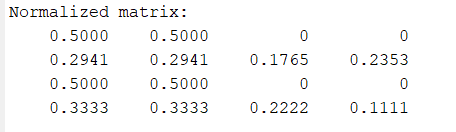
\includegraphics[width=1.0\textwidth]{norm_matrix.png}
    \caption{Нормированная матрица переходов}
\end{figure}

\begin{figure}[H]
    \centering
    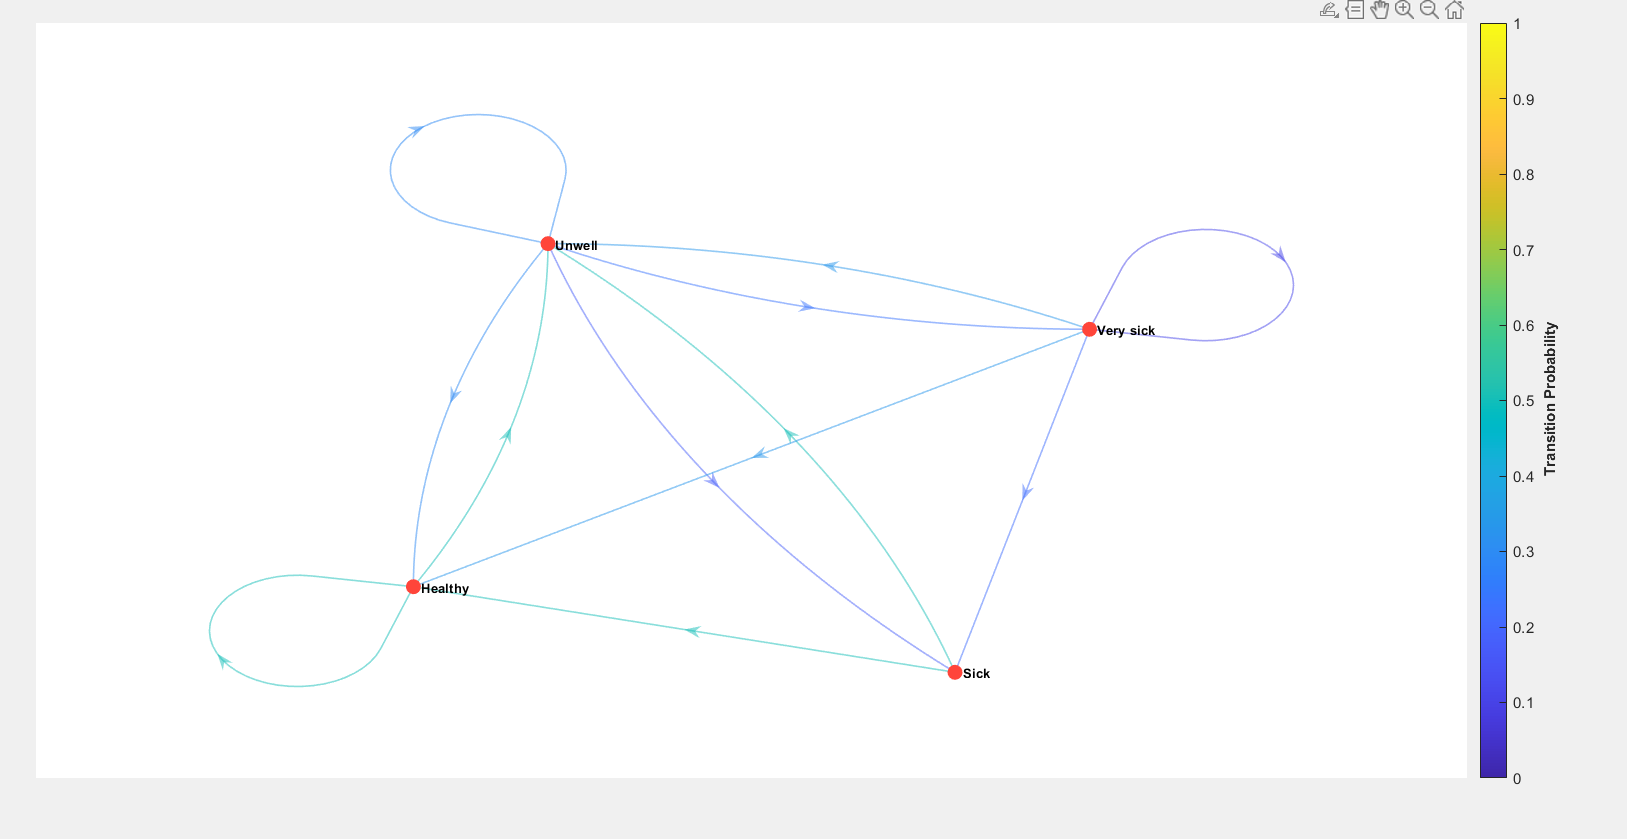
\includegraphics[width=1.0\textwidth]{markov_chain.png}
    \caption{Представление цепи Маркова в виде графа}
\end{figure}

Данный граф отражает, сколько состояний у системы, как состояния связаны между собой и с какой вероятностью могут переходить в 
другие состояния. \\

С помощью встроенной функции созадим кумулятивную матрицу - матрицу, в каждой строке которой каждое значение является суммой всех 
предыдущих. Если сумма становится > 1, то значение округляется до 1.

\begin{figure}[H]
    \centering
    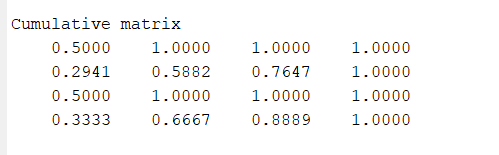
\includegraphics[width=1.0\textwidth]{cum_matrix.png}
    \caption{Кумулятивная матрица}
\end{figure}

Эта матрица нам нужна будет в дальнейшем для моделирования переходов в цепи Маркова \\

Реализуем алгоритм, моделирующий переходы в цепи Маркова:

\begin{figure}[H]
    \centering
    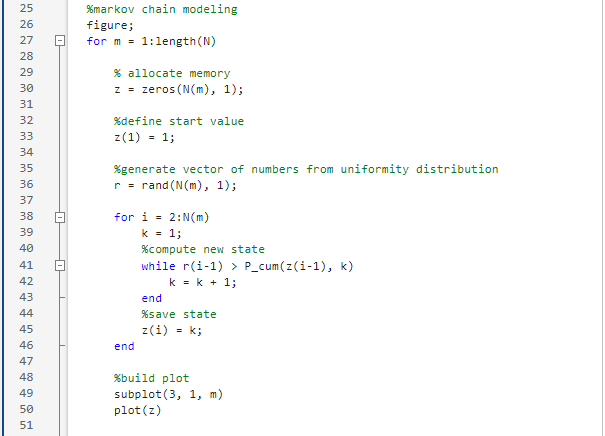
\includegraphics[width=1.0\textwidth]{markov modeling.png}
    \caption{Алгоритм моделировани цепи Маркова}
\end{figure}

В данном алгоритме сначала задается начальное значение z(1) = 1. Это показывает, в каком состоянии (вершине графа) находится
система на начало моделирования. Далее будем сравнивать вероятность перехода в другую вершину (пробегаемся по строке) с 
числом из отрезка [0;1] сгенерированного по законам нормального расрпеделения. Это делается потому, что марковский процесс
случаен, т.е нет правила переходов между состояниями, есть только вероятность, с которой это можно сделать. Сравнение со 
случайным числом как раз вносит эту самую случайность при моделировании. Вычисляем следующую вершину и сохраняем для последующих
вычислений.\\

Результаты моделирования для N = 200, 1000, 10000. N - кол-во временных отсчетов или кол-во переходов:

\begin{figure}[H]
    \centering
    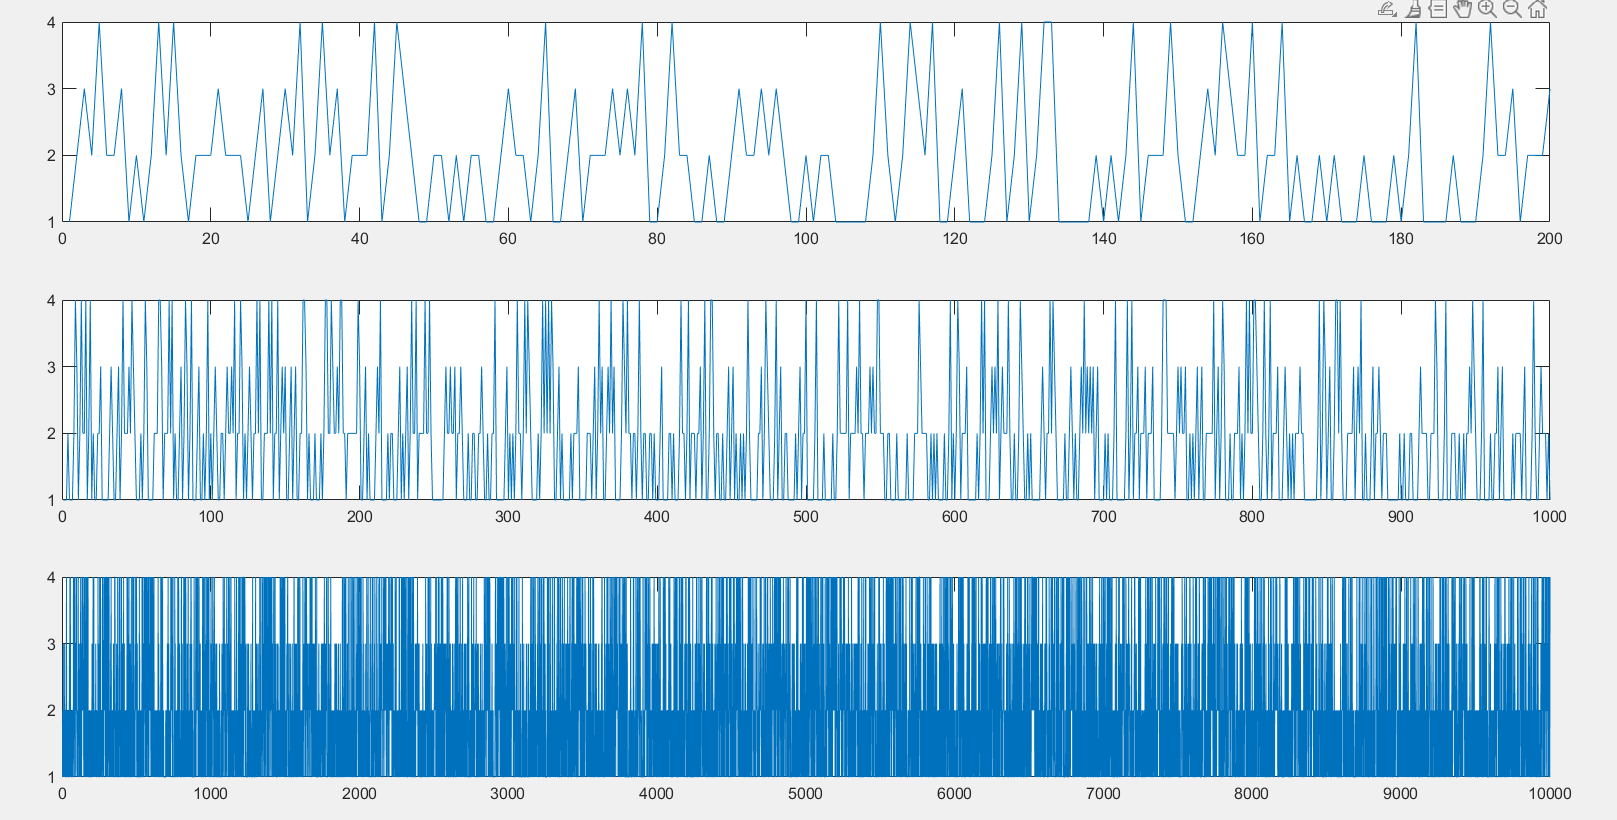
\includegraphics[width=1.0\textwidth]{modeling_result.png}
    \caption{Результаты моделирования}
\end{figure}

На графиках по оси Y отложены состояния системы, а по оси X - временные отсчеты. График иллюстрирует переходы в цепи Маркова. \\

Вычислим оценку цепи Маркова:

\begin{figure}[H]
    \centering
    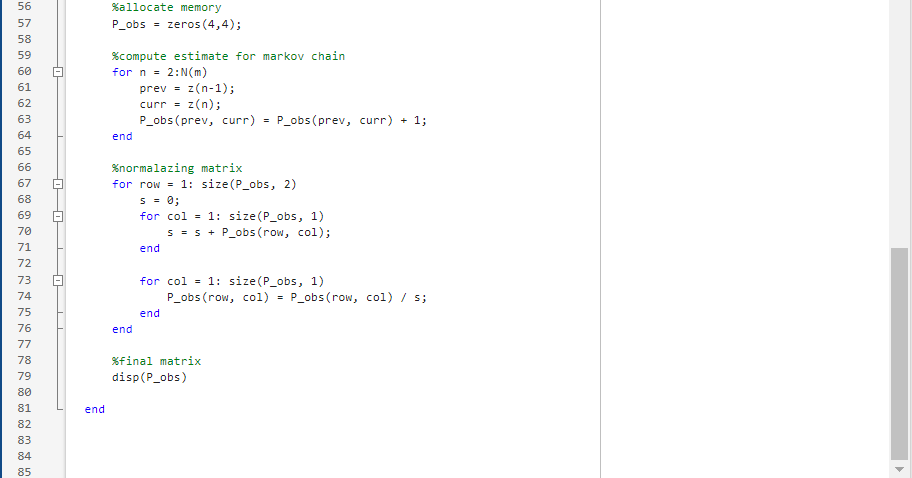
\includegraphics[width=1.0\textwidth]{markov_estim.png}
    \caption{Алгоритм оценки цепи Маркова}
\end{figure}

Данный алгоритм по сути вычисляет, сколько раз было сделано переходов в то или иное состояние системы, а потом нормализует
полученную матрицу. \\

Результат:

\begin{figure}[H]
    \centering
    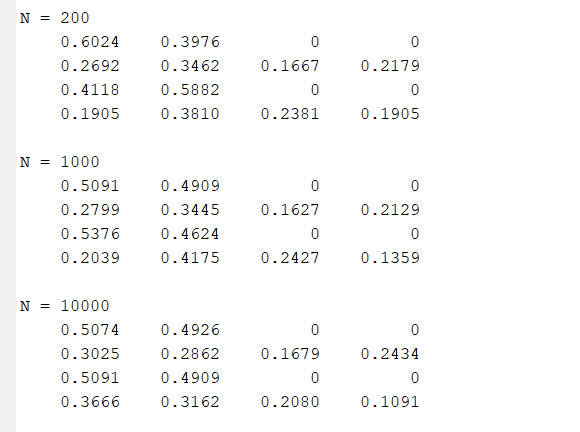
\includegraphics[width=1.0\textwidth]{estim_result.png}
    \caption{Оценка цепи Маркова}
\end{figure}

Можем заметить, что данная матрица очень похожа на исходную матрицу переходов, причем с увеличением N матрица становится всё более
похожей на исходную. Это говорит о том, что система, построенная по законам цепи Маркова со временем сохраняет свои начальные 
характеристики (матрицу переходов).

\section*{\textbf{Расчет характеристик СМО}}

Реализация:

\begin{figure}[H]
    \centering
    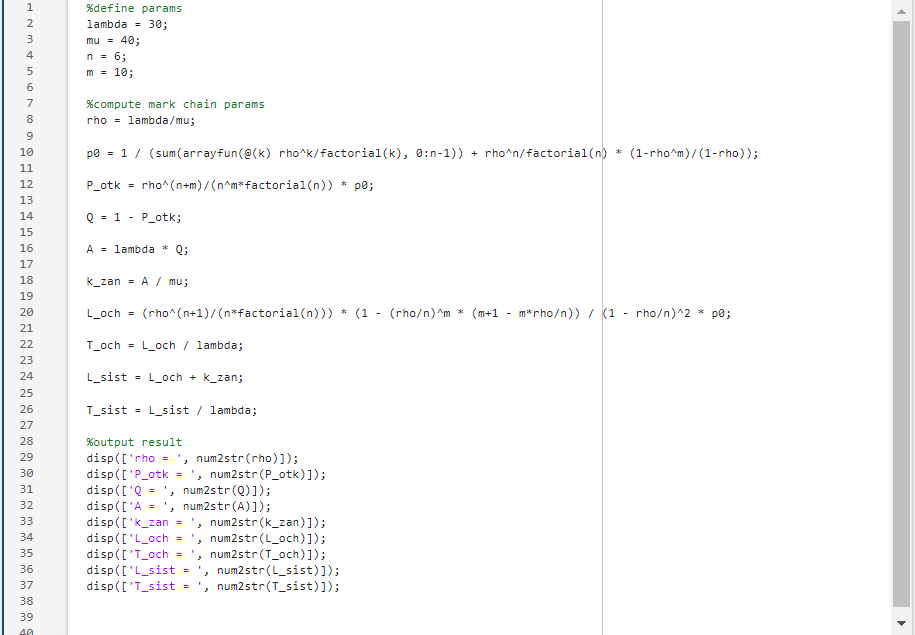
\includegraphics[width=1.0\textwidth]{params.png}
    \caption{Расчет параметров СМО}
\end{figure}

Результат:

\begin{figure}[H]
    \centering
    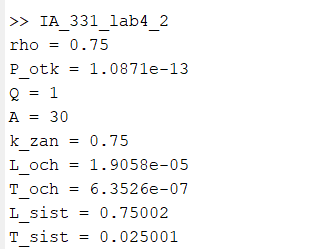
\includegraphics[width=1.0\textwidth]{params_result.png}
    \caption{Результат расчетов}
\end{figure}

Как результаты характеризуют такую СМО? \\

Такая СМО имеет большую пропускную способность (A) относительно среднего кол-ва заявок (Q), из это следует малые среднее количество занятых каналов (kзан),
среднее количество заявок в системе (Lсист), среднее время пребывания заявки в системе (Tсист), средняя длина очереди (Lоч), 
среднее время ожидания заявки в очереди (Tоч) и малая вероятность отказа.


\section*{\textbf{Пример СМО в simulink}}

\begin{figure}[H]
    \centering
    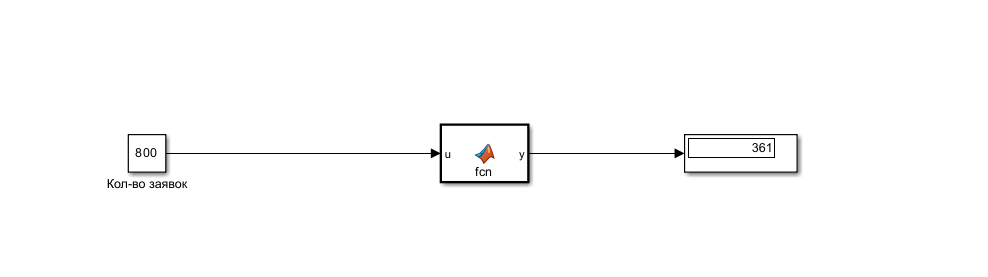
\includegraphics[width=1.0\textwidth]{smo_examp.png}
    \caption{Пример системы массового обслуживания}
\end{figure}

Блок с константой - число заявок, поданых на СМО. Саму логику СМО реализует функция-блок и кол-во обслуженных заявок передает на
display. \\

Реализация функции-блока:

\begin{figure}[H]
    \centering
    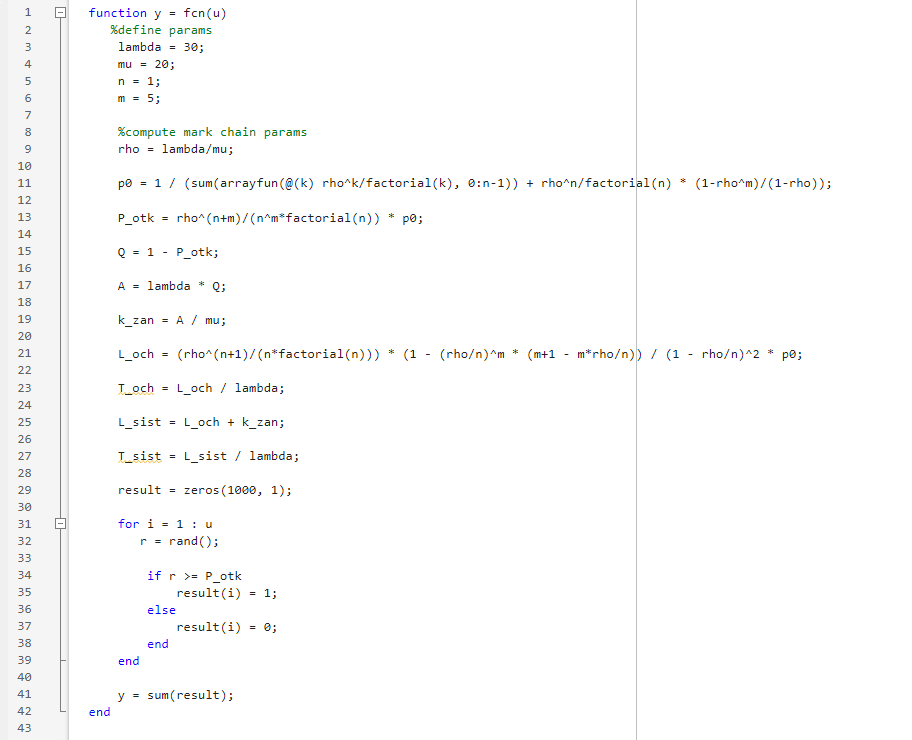
\includegraphics[width=1.0\textwidth]{func_block.png}
    \caption{Реализация СМО}
\end{figure}

В функции задаются начальные параметры, из которых высчитываются остальные. Самый важный параметр - вероятность отказа. Функция
с вероятностью $P_{отк}$ либо обслуживает клиента, либо нет. Можно поиграться с параметрами и смотреть, как будет вести себя система.
Можно сделать логику сложнее, чтобы участвовал не один параметр, а несколько. \\

Увеличим число каналов работы СМО и посмотрим, как это отразится на результате:

\begin{figure}[H]
    \centering
    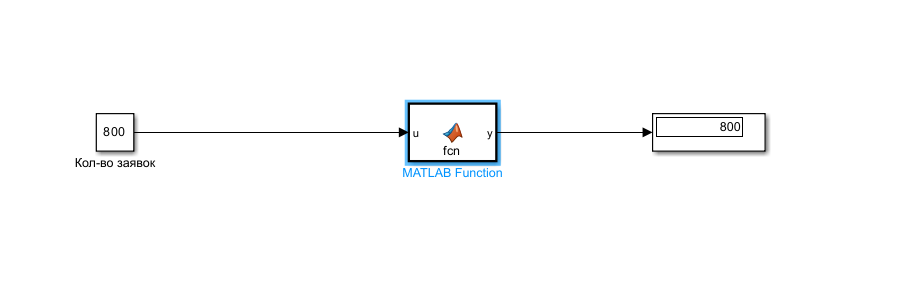
\includegraphics[width=1.0\textwidth]{up_channel.png}
    \caption{Зависимость работы СМО от кол-ва каналов}
\end{figure}

Видим, что при увеличении числа каналов до 6 (до этого был всего один) вероятность обработать заявку кратно выросла.

\endinput
